%!TEX root = /Users/louis/Documents/PhD/Deliverables/Thesis/thesis.tex

\section{Epsilon Flock: A Model Migration Language}
\label{sec:flock}
Driven by the analysis presented above, a domain-specific language for model migration, Epsilon Flock (subsequently referred to as Flock), was designed and implemented. Section~\ref{subsec:flock_design} discusses the principle tenets of Flock, including the way in which automatically maps each element of the original model to an equivalent element of the migrated model using a novel conservative copying algorithm and user-defined migration rules. In Section~\ref{subsec:flock_examples}, Flock is demonstrated via application to two examples of model migration. The work described in this section has been published in \cite{rose10flock}.


\subsection{Design and Implementation}
\label{subsec:flock_design}
Flock is a rule-based transformation language that mixes declarative and imperative parts. Its style is inspired by hybrid model-to-model transformation languages such as the Atlas Transformation Language \cite{jouault05transforming} and the Epsilon Transformation Language \cite{kolovos08etl}. Flock has a compact syntax. Much of its design and implementation is focused on the runtime. The way in which Flock relates source to target elements is novel; it is neither a new nor an existing target relationship. Instead, elements are copied conservatively, as described in Section~\ref{subsubsec:conservative_copying}.

Like Epsilon HUTN (\ref{subsec:epsilon_hutn}), Flock is built atop Epsilon, which was described in Section~\ref{subsec:epsilon}. In particular, Flock uses the model connectivity layer and the object language of Epsilon. The former is used to decouple migration from the representation of models and to provide compatibility with several modelling frameworks, while the latter provides a language for specifying user-defined migration rules, which are now discussed. 

\subsubsection{Abstract Syntax}
\label{subsubsec:abstract_syntax}
As illustrated by Figure~\ref{fig:abstract_syntax}, Flock migration strategies are organised into modules (\texttt{Fl\-ockMo\-du\-le}), which inherit from EOL modules (\texttt{Eo\-lMod\-ule}), which provides support for module reuse with import statements and user-defined operations. Modules comprise any number of rules (\texttt{Ru\-le}). Each rule has an original metamodel type (\texttt{or\-ig\-in\-alTy\-pe}) and can optionally specify a \texttt{gu\-ard}, which is either an EOL statement or a block of EOL statements. \texttt{Mi\-gr\-ateRu\-le}s must specify an evolved metamodel type (\texttt{ev\-ol\-vedTy\-pe}) and/or a \texttt{bo\-dy} comprising a block of EOL statements.

\begin{figure}
  \centering
  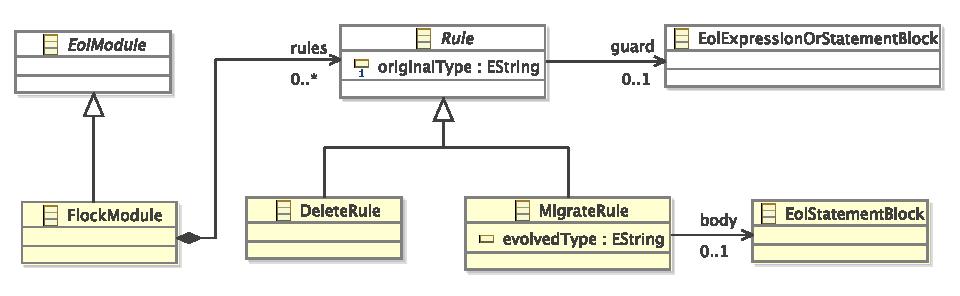
\includegraphics[scale=0.75]{5.Implementation/flock_abstract_syntax.pdf}
  \caption{The abstract syntax of Flock.}
  \label{fig:abstract_syntax}
\end{figure}

\subsubsection{Concrete Syntax}
\label{subsubsec:concrete_syntax}

Listing~\ref{lst:flock_concrete_syntax} shows the concrete syntax of migrate and delete rules. All rules begin with a keyword indicating their type (either \texttt{migrate} or \texttt{delete}), followed by the original metamodel type. Guards are specified using the \texttt{when} keywords. Migrate rules may also specify an evolved metamodel type using the \texttt{to} keyword and a \texttt{body} as a (possibly empty) sequence of EOL statements.

Note there is presently no create rule. In Flock, the creation of new model elements is usually encoded in the imperative part of a migrate rule specified on the containing type.

\begin{lstlisting}[float=tbp, caption=Concrete syntax of migrate and delete rules., label=lst:flock_concrete_syntax, language=Flock]
migrate <originalType> (to <evolvedType>)?
(when (:<eolExpression>)|({<eolStatement>+}))? {
	<eolStatement>*
} 

delete <originalType>
(when (:<eolExpression>)|({<eolStatement>+}))?
\end{lstlisting}

\subsubsection{Execution Semantics}
A Flock module has the following behaviour when executed:

\begin{enumerate}
	\item For each original model element, \texttt{e}:
	\subitem Identify an applicable rule, \texttt{r}. To be applicable for \texttt{e}, a rule must have as its original type the metaclass (or a supertype of the metaclass) of \texttt{e} and the guard part of the rule must be satisfied by \texttt{e}.
	\subitem When no rule can be applied, a default rule is used, which has the metaclass of \texttt{e} as its original type, and an empty body.
	
	\item For each mapping between original model element, \texttt{e}, and applicable delete rule, \texttt{r}:
	\subitem Do nothing.
	
	\item For each mapping between original model element, \texttt{e}, and applicable migrate rule, \texttt{r}:
	\subitem Create an equivalent model element, \texttt{e'} in the migrated model. The metaclass of \texttt{e'} is determined from the \texttt{evolvedType} (or the \texttt{originalType} when no \texttt{evolvedType} has been specified) of \texttt{r}.
	\subitem Copy the data contained in \texttt{e} to \texttt{e'} (using the \emph{conservative copy} algorithm described in the sequel).

	\item For each mapping between original model element, \texttt{e}, applicable migrate rule, \texttt{r}, and equivalent model element, \texttt{e'}:
	\subitem Execute the body of \texttt{r} binding \texttt{e} and \texttt{e'} to variables named \texttt{original} and \texttt{migrated}, respectively.
\end{enumerate}


\subsubsection{Conservative Copying}
\label{subsubsec:conservative_copying}
% TODO A detailed example of conservative copy + equivalence establishment might be useful
Flock contributes an algorithm, termed \emph{conservative copy}, that copies model elements from original to migrated model only when those model elements conform to the evolved metamodel. Because of its conservative copy algorithm, Flock is a hybrid of new target and existing target transformation languages. This section discusses the conservative copying algorithm in more detail.

The algorithm operates on an original model element, \texttt{o}, and its equivalent model element in the migrated model, \texttt{e}. When \texttt{o} has no equivalent in the migrated model (for example, when a metaclass has been removed and the migration strategy specifies no alternative metaclass), \texttt{o} is not copied to the migrated model. Otherwise, conservative copy is invoked for \texttt{o} and \texttt{e}, proceeding as follows:

\begin{itemize}
	\item For each metafeature, \texttt{f} for which \texttt{o} has specified a value
		\subitem Locate a metafeature in the evolved metamodel with the same name as \texttt{f} for which \texttt{e} may specify a value.
			\subsubitem When no equivalent metafeature can be found, do nothing.
			\subsubitem Otherwise, copy to the migrated model the original value (\texttt{o.f}) only when it conforms to the equivalent metafeature
\end{itemize}

The definition of conformance varies over modelling frameworks. Typically, conformance between a value, \texttt{v}, and a feature, \texttt{f}, specifies at least the following constraints:

\begin{itemize}
	\item The size of \texttt{v} must be greater than or equal to the lowerbound of \texttt{f}.
	\item The size of \texttt{v} must be less than or equal to the upperbound of \texttt{f}.
	\item The type of \texttt{v} must be the same as or a subtype of the type of \texttt{f}.
\end{itemize}


Epsilon includes a model connectivity layer (EMC), which provides a common interface for accessing and persisting models. Currently, EMC provides drivers for several modelling frameworks, permitting management of models defined with EMF, the Metadata Repository (MDR), Z or XML. To support migration between metamodels defined in heterogenous modelling frameworks, EMC was extended during the development of Flock. The connectivity layer now provides a conformance checking service. Each EMC driver was extended to include conformance checking semantics specific to its modelling framework. Flock implements conservative copy by delegate conformance checking responsibilities to EMC. 

Finally, some categories of model value must be converted before being copied from the original to the migrated model. Again, the need for and semantics of this conversion varies over modelling frameworks. Reference values typically require conversion before copying. In this case, the mappings between original and migrated model elements maintained by the Flock runtime can be used to perform the conversion. In other cases, the target modelling framework must be used to perform the conversion, such as when EMF enumeration literals are to be copied.


\subsubsection{Development and User Tools}
As discussed in Section~\ref{sec:analysing_existing_techniques}, models and metamodels are typically kept separate. Flock migration strategies can be distributed by the metamodel developer in two ways. An extension point defined by Flock provides a generic user interface for migration strategy execution. Alternatively, metamodel developers can elect to build their own interface, delegating execution responsibility to \texttt{FlockModule}. We anticipate the latter to be useful for production environments using model or source code management repositories.


\subsection{Examples}
\label{subsec:flock_examples}
Flock is now demonstrated using two examples of model migration. Listing~\ref{lst:flock} illustrates the Flock migration strategy for the Petri net example introduced above and is included for direct comparison with other approaches. An additional, larger example is presented based on changes made to UML class diagrams between versions 1.5 and 2.0 of the UML specification.

\subsubsection{Petri Nets in Flock}
The exemplar Petri net metamodel evolution is now revisited to demonstrate the basic functionality of Flock. In Listing~\ref{lst:flock}, \texttt{Net}s and \texttt{Place}s are migrated automatically. Unlike the ATL migration strategy (Listing~\ref{lst:atl}), no explicit copying rules are required. Compared to the COPE migration strategy (Listing~\ref{lst:cope}), the Flock migration strategy does not explicitly unset the original \texttt{src} and \texttt{dst} features of \texttt{Transition}.

\begin{lstlisting}[caption=Petri nets model migration in Flock, label=lst:flock, language=Flock]
migrate Transition {
  for (source in original.src) {
    var arc := new Migrated!PTArc;
    arc.src := source.equivalent();  arc.dst := migrated;
    arc.net := original.net.equivalent();
  }

  for (destination in original.dst) {
    var arc := new Migrated!TPArc;
    arc.src := migrated;  arc.dst := destination.equivalent();
    arc.net := original.net.equivalent();
  }
}
\end{lstlisting}

\subsubsection{Petri Nets in Flock}
Figure~\ref{fig:uml_mms} illustrates a subset of the changes made between UML 1.5 and UML 2.0. Only class diagrams are considered, and features that did not change are omitted. In Figure~\ref{fig:original_uml_mm}, association ends and attributes are specified explicitly and separately. In Figure~\ref{fig:evolved_uml_mm}, the \texttt{Pr\-op\-er\-ty} class is used instead. The Flock migration strategy (Listing~\ref{lst:flock-uml}) for Figure~\ref{fig:uml_mms} is now discussed.

\begin{lstlisting}[caption=UML model migration in Flock, label=lst:flock-uml, language=Flock]
migrate Association {
	migrated.memberEnds := original.connections.equivalent();
}

migrate Class {
	var fs := original.features.equivalent();
	migrated.operations := fs.select(f|f.isKindOf(Operation));
	migrated.attributes := fs.select(f|f.isKindOf(Property));
	migrated.attributes.addAll(original.associations.equivalent())
}

delete StructuralFeature when: original.targetScope <> #instance

migrate Attribute to Property {
	if (original.ownerScope = #classifier) {
		migrated.isStatic = true;		
	}
}
migrate Operation {
	if (original.ownerScope = #classifier) {
		migrated.isStatic = true;
	}
}

migrate AssociationEnd to Property {
	if (original.isNavigable) {
		original.association.equivalent().navigableEnds.add(migrated)
	}
}
\end{lstlisting}

Firstly, \texttt{At\-tr\-ib\-ut\-e}s and \texttt{As\-so\-ci\-at\-i\-onEn\-d}s are now modelled as \texttt{Pr\-o\-pe\-rt\-ies} (lines 16 and 28). In addition, the \texttt{As\-so\-ci\-at\-i\-on\#na\-vi\-ga\-b\-leEn\-ds} reference replaces the \texttt{As\-so\-ci\-at\-i\-onE\-nd\#isN\-av\-ig\-ab\-le} attribute; following migration, each navigable \texttt{As\-so\-ci\-at\-i\-onE\-nd} must be referenced via the \texttt{na\-vi\-ga\-bl\-eEn\-ds} feature of its \texttt{As\-so\-ci\-at\-ion} (lines 29-31).

In UML 2.0, \texttt{St\-ru\-ct\-ur\-alFe\-at\-ur\-e\#o\-wn\-er\-Sc\-op\-e} has been replaced by \texttt{\#i\-sS\-ta\-ti\-c} (lines 17-19 and 23-25). The UML 2.0 specification states that \texttt{Sc\-op\-eKi\-nd\#cl\-as\-si\-fi\-er} should be mapped to true, and \texttt{\#i\-ns\-ta\-nce} to false. 

The UML 1.5 \texttt{St\-ru\-ct\-ur\-alFe\-at\-ur\-e\#t\-ar\-g\-et\-Sc\-op\-e} feature is no longer supported in UML 2.0, and no migration path is provided. Consequently, line 14 deletes any model element whose \texttt{t\-ar\-g\-et\-Sc\-op\-e} is not the default value.

\begin{figure}
	\centering
	\subfigure[Original metamodel.]
	{
	    \label{fig:original_uml_mm}
	    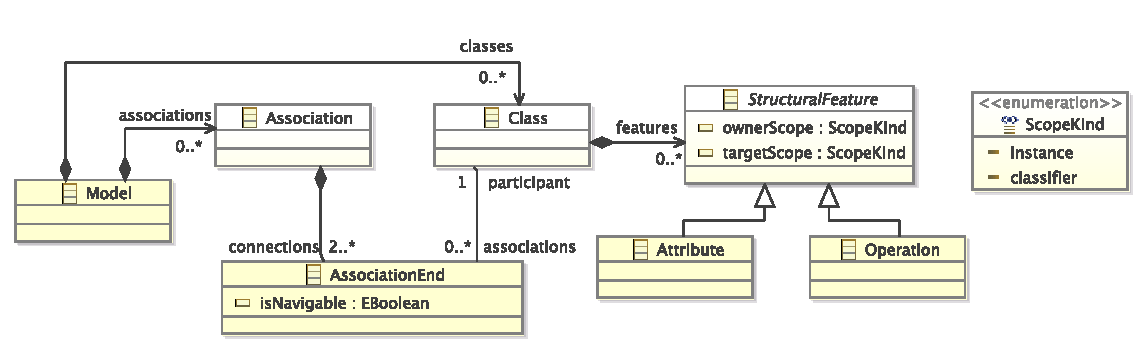
\includegraphics[width=10.5cm]{5.Implementation/uml_step0.pdf}
	}
	\subfigure[Evolved metamodel.]
	{
	    \label{fig:evolved_uml_mm}
	    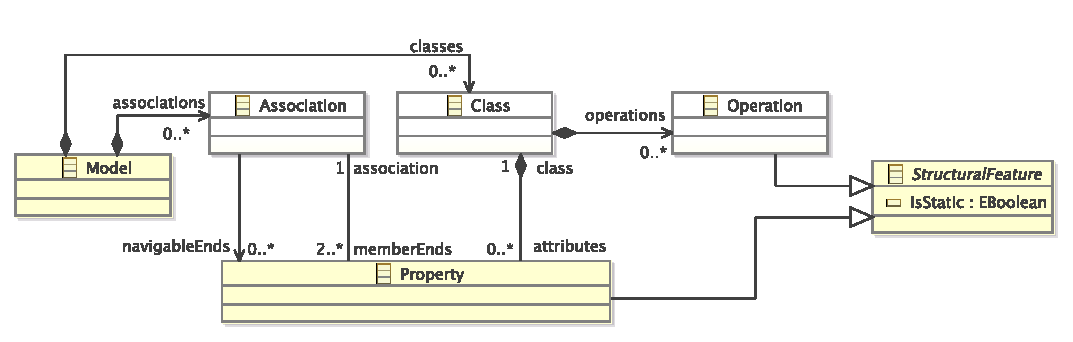
\includegraphics[width=10.5cm]{5.Implementation/uml_step1.pdf}
	}
	\caption[Exemplar UML metamodel evolution]{Exemplar UML metamodel evolution. (Shading is irrelevant).}
\label{fig:uml_mms}
\end{figure}

Finally, \texttt{C\-la\-ss\#fe\-at\-ur\-es} has been split to form \texttt{C\-la\-ss\#op\-er\-at\-io\-ns} and \texttt{\#at\-tr\-ib\-ut\-es}. Lines 8 and 10 partition features on the original \texttt{Cl\-a\-ss}. \texttt{Cl\-as\-s\#a\-ss\-oc\-ia\-ti\-on\-s} has been removed in UML 2.0, and \texttt{As\-so\-ci\-at\-i\-onEn\-d}s are instead stored in \texttt{Cl\-a\-ss\#at\-tr\-ib\-ut\-es} (line 11).


\subsubsection{Comparison}
Table~\ref{tab:differences} illustrates several characterising differences between Flock and the related approaches presented in Section~\ref{subsec:co-evo_example}. Due to its conservative copying algorithm, Flock is the only approach to provide both automatic copying and unsetting. Automatic copying is significant for metamodel evolutions with a large number of unchanging features.

All of the approaches considered in Table~\ref{tab:differences} support EMF, arguably the most widely used modelling framework. The Ecore2Ecore approach, however, requires migration to be encoded at the level of the underlying model representation XMI. Both Flock and ATL support other modelling technologies, such as MDR and XML. However, ATL does not automatically copy model elements that have not been affected by metamodel changes. Therefore, migration between models of different technologies with ATL requires extra statements in the migration strategy to ensure that the conformance constraints of the target technology are satisfied. Because it delegates conformance checking to an EMC driver, Flock requires no such checks.

\begin{table}[b]
	\caption{Properties of model migration approaches}
	\centering
	\begin{tabular}{|c|c|c|c|}
		\hline
		             & \textbf{Automatic copy} & \textbf{Automatic unset} & \textbf{Modelling technologies} \\
		\hline
		\textbf{Ecore2Ecore}  & \tick             & \cross              & XMI                    \\
		\hline
		\textbf{ATL}          & \cross            & \tick               & EMF, MDR, KM3, XML     \\
		\hline
		\textbf{COPE}         & \tick             & \cross              & EMF                    \\
		\hline
		\textbf{Flock}        & \tick             & \tick               & EMF, MDR, XML, Z       \\
		\hline
	\end{tabular}
	\label{tab:differences}
\end{table}

A more thorough examination of the similarities and differences between Flock and other migration strategy languages is provided in Chapter~\ref{Evaluation}.
